\documentclass[10pt,a4paper]{article}
\usepackage[utf8]{inputenc}

\usepackage[landscape,margin=1cm]{geometry}
\usepackage[english]{babel}


% colour themes to come. KnitR?

%-------------------------

\title{\color{w3schools}Yaml Cheatsheet
}
%\author{Abdelkader Amar}
%\date{\today}

\usepackage{colourful_updated_template}

% \usepackage[default]{raleway}
\usepackage{fontawesome}
\usepackage[T1]{fontenc}

\usepackage{hyperref}
\usepackage{enumitem}
\usepackage{lipsum}

\usepackage{xcolor}
\definecolor{customcolor}{HTML}{696EA8} %  616AC5
\definecolor{alert}{HTML}{CD5C5C}
\definecolor{w3schools}{HTML}{4CAF50}
\definecolor{subbox}{gray}{0.60}
\definecolor{codecolor}{HTML}{FFC300} % altes Ocker



%--------------------------------------------------------------------------------
% from metropolis theme
\definecolor{mDarkTeal}{HTML}{23373b}
\colorlet{beamerboxbg}{black!2}
\colorlet{beamerboxfg}{mDarkTeal}
\definecolor{mDarkBrown}{HTML}{604c38}
\definecolor{mDarkTeal}{HTML}{23373b}
\definecolor{mLightBrown}{HTML}{EB811B}
\definecolor{mLightGreen}{HTML}{14B03D}
\definecolor{alertTextBox}{HTML}{A8696E}
% https://htmlcolorcodes.com/color-picker/ --> take 696EA8 for a spin
%--------------------------------------------------------------------------------
%\colorlet{codecolor}{mDarkTeal!60}

%--------------------------Editor mode.

\usepackage
[citestyle=authoryear,
sorting=nty,	  		%Sorts bibliography by year, name, title
autocite=footnote, 		%Autocite command generates footnotes
autolang=hyphen, 		
mincrossrefs=1, 	
backend=biber]
{biblatex}

\DeclareFieldFormat{postnote}{#1}
\DeclareFieldFormat{multipostnote}{#1}
\DeclareAutoCiteCommand{footnote}[f]{\footcite}{\footcites}

\bibliography{literature}
%----------------------------------------
%--------------------------------------------------------------------------------
\usepackage{tcolorbox}

\tcbuselibrary{most,listingsutf8,minted}

\tcbset{tcbox width=auto,left=1mm,top=1mm,bottom=1mm,
right=1mm,boxsep=1mm,middle=1pt}

\newenvironment{mycolorbox}[2]{%
\begin{tcolorbox}[grow to left by=-1em,grow to right by=-1em,capture=minipage,fonttitle=\large\bfseries, enhanced jigsaw,boxsep=1mm,colback=#1!30!white,on line,tcbox width=auto,
arc=2pt,outer arc=2pt, % 0pt = eckig
toptitle=0mm,colframe=#1,opacityback=0.7,nobeforeafter,title=#2]%
}{\end{tcolorbox}\\[0.2em]}

\newenvironment{subbox}[2]{%
\begin{tcolorbox}[capture=minipage,fonttitle=\normalsize\bfseries, enhanced jigsaw,boxsep=1mm,colback=#1!30!white,on line,tcbox width=auto,left=0.3em,top=1mm, toptitle=0mm,colframe=#1,opacityback=0.7,nobeforeafter,title=#2]\footnotesize %
}{\normalsize\end{tcolorbox}\vspace{0.1em}}

\newenvironment{multibox}[1]{%
\begin{tcbraster}[raster columns=#1,raster equal height,nobeforeafter,raster column skip=1em,raster left skip=1em,raster right skip=1em]}{\end{tcbraster}}

\newenvironment{textbox}[1]{\begin{mycolorbox}{customcolor}{#1}}{\end{mycolorbox}}
\newenvironment{alerttextbox}[1]{\begin{mycolorbox}{alertTextBox}{#1}}{\end{mycolorbox}}


%-------------------------------
\newtcblisting{oldcodebox}[2]{colback=codecolor!5,colframe=codecolor!80!black,listing only, 
minted options={numbers=left,style=tcblatex,fontsize=\tiny,breaklines,autogobble,linenos,numbersep=3mm},
left=5mm,enhanced,
title=#2, fonttitle=\bfseries,
listing engine=minted,minted language=#1}

%--------------------------------------------------------------------------------
\newcommand{\punkti}{~\lbrack\dots\rbrack~}

\renewenvironment{quote}
               {\list{\faQuoteLeft\phantom{ }}{\rightmargin\leftmargin}%
                \item\relax\scriptsize\ignorespaces}
               {\unskip\unskip\phantom{xx}\faQuoteRight\endlist}
               

%--------------------------------------------------------------------------------
\newcommand{\bgupper}[3]{\colorbox{#1}{\color{#2}\huge\bfseries\MakeUppercase{#3}}}
\newcommand{\bg}[3]{\colorbox{#1}{\bfseries\color{#2}#3}}

\newcommand{\mycommand}[2]{{\ttfamily\detokenize{#1}}~\dotfill{}~{#2}\\}
% urspr war hier vor #2 \footnotesize
\newcommand{\sep}{{\scriptsize~\faCircle{ }~}}


\newcommand{\bggreen}[1]{\medskip\bgupper{w3schools}{black}{#1}\\[0.5em]}
\newcommand{\green}[1]{\smallskip\bg{w3schools}{white}{#1}\\}
\newcommand{\red}[1]{\smallskip\bg{alert}{white}{#1}\\}
\newcommand{\alert}[1]{\red{#1}\\}

\usepackage{multicol}
\setlength{\columnsep}{30pt}

\setlength{\parindent}{0pt}
\pagestyle{empty}

\usepackage{csquotes}

\newcommand{\loremipsum}{Lorem ipsum dolor sit amet.}



%--------------------------------------------------------------------------------
% https://tex.stackexchange.com/questions/2504/beamer-blocks-in-ordinary-article-style-document
% just adding beamerblocks for definitions

%--------------------------------------------------------------------------------
\newenvironment{myexampleblock}[1]{%
    \tcolorbox[capture=minipage,fonttitle=\small\bfseries\color{mLightGreen}, enhanced jigsaw,boxsep=1mm,colback=black!10,breakable,noparskip,
    on line,tcbox width=auto,left=0.3em,top=1mm, toptitle=0mm,
    colframe=black!20,arc=0pt,outer arc=0pt,
    opacityback=0.7,nobeforeafter,title=#1]}%
    {\endtcolorbox}
    
\newenvironment{myalertblock}[1]{%
    \tcolorbox[capture=minipage,fonttitle=\small\bfseries\color{mLightBrown}, enhanced jigsaw,boxsep=1mm,colback=black!10,breakable,noparskip,
    on line,tcbox width=auto,left=0.3em,top=1mm, toptitle=0mm,
    colframe=black!20,arc=0pt,outer arc=0pt,
    opacityback=0.7,nobeforeafter,title=#1]}%
    {\endtcolorbox}

\newenvironment{myblock}[1]{%
    \tcolorbox[capture=minipage,fonttitle=\small\bfseries\color{mDarkTeal}, enhanced jigsaw,boxsep=1mm,colback=black!10,breakable,noparskip,
    on line,tcbox width=auto,left=0.3em,top=1mm, toptitle=0mm,
    colframe=black!20, arc=0pt,outer arc=0pt,
    opacityback=0.7,nobeforeafter,title=#1]}%
    {\endtcolorbox}
    
%-------------------------------
\newtcblisting{Xcodebox}[2]{colback=black!10,colframe=black!20,
listing only, 
minted options={numbers=left,style=tcblatex,fontsize=\scriptsize,
breaklines,autogobble,linenos,numbersep=6pt,framesep=3mm},
enhanced,left=0.3em,top=1mm, toptitle=0mm, 
arc=0pt,outer arc=0pt,
title=#2, fonttitle=\small\bfseries\color{mDarkTeal},
listing engine=minted,minted language=#1}

%https://tex.stackexchange.com/questions/324863/line-numbering-column-colorization
\newtcblisting{codebox}[2]{colback=black!10,colframe=black!20,
listing only, 
minted options={numbers=left, style=tcblatex,fontsize=\scriptsize,breaklines,
breaksymbolleft=,autogobble,linenos,numbersep=0.7em},
enhanced,top=1mm, toptitle=0mm, 
left=5mm,
arc=0pt,outer arc=0pt,
title=#2, fonttitle=\small\bfseries\color{mDarkTeal},
listing engine=minted,minted language=#1}


%--------------------------------------------------------------------------------
% from tcolorbox: https://mirror.easyname.at/ctan/macros/latex/contrib/tcolorbox/tcolorbox.pdf
\newcommand{\mygraphics}[2][]{%
\tcbox[enhanced,boxsep=0pt,top=0pt,bottom=0pt,left=0pt,
right=0pt,boxrule=0.4pt,drop fuzzy shadow,clip upper,
colback=black!75!white,toptitle=2pt,bottomtitle=2pt,nobeforeafter,
center title,fonttitle=\small\sffamily,title=\detokenize{#2}]%
{\includegraphics[width=\the\dimexpr(\linewidth-4mm)\relax]{#2}}%
}
% {\includegraphics[width=\the\dimexpr(\linewidth-4mm)/2\relax]{#2}}}
%\mygraphics{lichtspiel.jpg}\hfill\mygraphics{Basilica_5.png}



%--------------------------------------------------------------------------------
\begin{document}
\maketitle
\small
\begin{multicols}{3}

\thispagestyle{empty}
%\maketitle
\scriptsize
%\tableofcontents

%-----------------------------------------------------
% \section{Preliminary Information}
%-----------------------------------------------------
%-----------------------------------------------------
% \subsection{Cheatsheet Examples}
% 
\begin{textbox}{Key concepts I}
\red{Bag-of-words (BOW)}

\green{\emph{type} vs. \emph{token}}
\emph{To be or not to be.} = 6 \emph{tokens}, 4 \emph{types}.

\red{\emph{type}} descriptive criterion\footcite[cf.][12]{stroustrup}

\red{\emph{token}} unit of analysis\footcites[cf.][12]{stroustrup,attentionMerchants}


\bigskip

\underline{Key topics}
\begin{itemize}
    \item One
    \item Two
    \item Three
\end{itemize}

\end{textbox}









%--------------------------------------------------------------
\section{Tools}



\begin{textbox}{Lorem Ipsum}
test  \sep test \sep test \sep test

\bigskip

\green{Visualize}
\begin{enumerate}
\item \textbf{present} your data
\item \textbf{analyze} the information
\item \textbf{explore} the findings
\end{enumerate}

\end{textbox}


\begin{textbox}{Voyant Tools}
 \href{https://voyant-tools.org/}{Voyant Tools} \sep \href{https://voyant-tools.org/}{Voyant Tools}

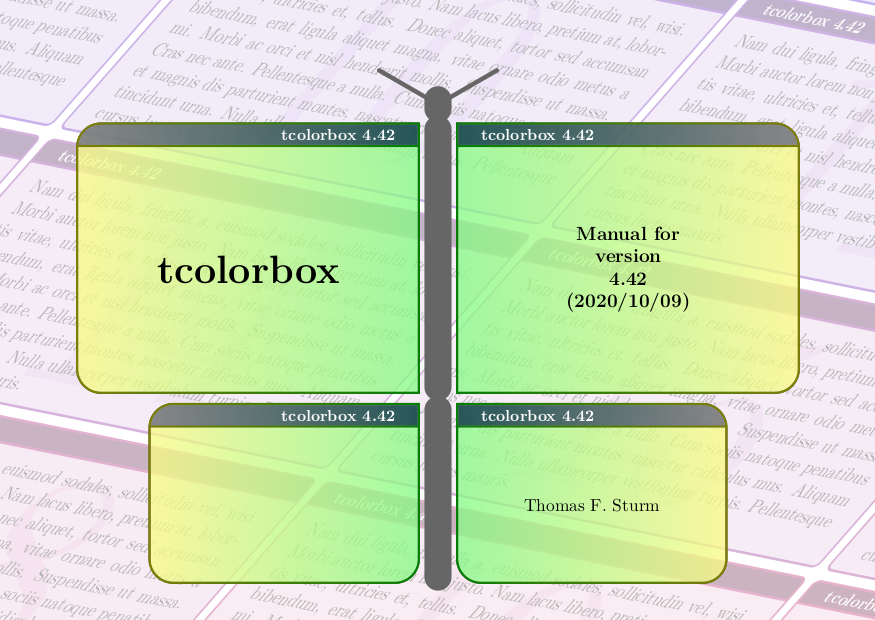
\includegraphics[width=\textwidth]{img/example-image.png}
\end{textbox}




\begin{textbox}{Project Gutenberg Texts}
\begin{tabular}{r|p{0.8\textwidth}}\scriptsize
    84 & \href{http://www.gutenberg.org/ebooks/84}{Frankenstein; Or, The Modern Prometheus by Mary Wollstonecraft Shelley} \\
    6087 & \href{https://www.gutenberg.org/ebooks/6087}{The Vampyre; a Tale by John William Polidori} \\
    696 & \href{https://www.gutenberg.org/ebooks/696}{The Castle of Otranto by Horace Walpole} \\
    42 & \href{https://www.gutenberg.org/ebooks/42}{The Strange Case of Dr. Jekyll and Mr. Hyde by Robert Louis Stevenson}
\end{tabular}

\end{textbox}





\begin{textbox}{Key concepts}
\red{Bag-of-words (BOW)}


\green{\emph{Zipf's Law}}

\mycommand{_&§!$§/()$}{code}
\mycommand{shutdown -h now}{to shutdown}

\end{textbox}


%--------------------------------------------------------------
\section{Programming}

\subsection{Code boxes}


% first argument: minted programming language name, for example.. css, c, cpp, etc.
\begin{codebox}{r}{Code box using R}
# Install
install.packages("tm")  # for text mining

# Load
library("tm")

# text <- readLines(file.choose())
# Read the text file from internet
filePath <- "http://www.internet.com/text.txt"
text <- readLines(filePath)

\end{codebox}


% first argument: minted programming language name, for example.. css, c, cpp, etc.
\begin{codebox}{cpp}{Code box using C++}
for (auto element : vector) 
{
    sum += element;
}
\end{codebox}

\section{Graphics}
The following is an example for a custom graphics command

\mygraphics{img/example-image.png}



\section{Other types of boxes}

\begin{alerttextbox}{The Alert Block}
\lipsum[10]
\end{alerttextbox}

\begin{myexampleblock}{The Example Block}
\lipsum[22]
\end{myexampleblock}

\mycommand{https://github.com}{Github Link Example}

\begin{myblock}{Branch}
Explanation
\end{myblock}

\begin{myblock}{Commit}
What's a commit?
\end{myblock}


\begin{myblock}{Staging}
s. Index
\end{myblock}


\begin{myblock}{Lipsum}
\lipsum[55]
\end{myblock}

\begin{textbox}{Yay Quotes}

\begin{quote}
    Yay, a quote!
\end{quote}

\begin{quote}
    Yay, a longer quote! \lipsum[5]
\end{quote}
\end{textbox}




\begin{codebox}{cpp}{multiline string}
Multilines value transformed to one line with eol added at the end
key: >
Multilines value transformed to one line without eol added at the end
key: >-
Multilines value kept unchanged with eol added at the end
key: |
Multilines value kept unchanged without eol at the end.
key: |-

\end{codebox}


%---------------------------------------------
\AtNextBibliography{\footnotesize}
\printbibliography  
\end{multicols}

\end{document}
